
\documentclass{article}

% Required packages
\usepackage{amssymb}
\usepackage{amsmath}
\usepackage{graphicx}
\usepackage{geometry}
\usepackage{tikz}
\usepackage{array}
\usepackage{booktabs}
\usepackage{enumitem}
\usepackage{listings}
\usepackage{xcolor}

% Set page geometry
\geometry{a4paper, margin=1in}

% Configure listings for Python
\lstset{
  language=Python,
  basicstyle=\ttfamily\footnotesize,
  numbers=left,
  numberstyle=\tiny\color{gray},
  frame=single,
  breaklines=true,
  breakatwhitespace=true,
  captionpos=b,
  tabsize=4,
  showspaces=false,
  showstringspaces=false,
  showtabs=false,
  commentstyle=\color{gray}\textit,
  keywordstyle=\color{blue}\bfseries,
  stringstyle=\color{red}
}

% For centering images and tables
\usepackage{float}

\begin{document}

\begin{flushright}
   Randall Rogers\\
   DSC 255: Machine Learning Fundamentals\\
   Homework 1: Nearest Neighbor Classification\\
   Spring 2025 \\
\end{flushright}

\subsection*{Question 1}
\textit{Casting an image into vector form. A $10 \times 10$ greyscale image is mapped to a $d$-dimensional vector, with one pixel per coordinate. What is $d$?}\\

\textbf{Solution} 

\noindent\rule{\textwidth}{0.4pt}\\

Let $l = 10$ ; $w = 10$ ; $d = l \times w$

Now, calculate the number of dimensions $d$.

$d = l \times w$

$d = 10 \times 10$

$d = 100$
   
$\therefore$ a $10 \times 10$ greyscale image is mapped to a $100$-dimensional vector\\

\noindent\rule{\textwidth}{0.4pt}
\noindent\rule{\textwidth}{0.4pt}

\subsection*{Question 2}

\textit{The length of a vector. The Euclidean (or $L_2$) length of a vector $x \in \mathbb{R}^d$ is}
$$
\|x\| = \sqrt{\sum_{i=1}^{d} x_i^2}
$$
\textit{where $x_i$ is the $i$-th coordinate of $x$. This is the same as the Euclidean distance between $x$ and the origin. What is the length of the vector which has a 1 in every coordinate? Your answer may be a function of $d$.}\\

\textbf{Solution} 

\noindent\rule{\textwidth}{0.4pt}\\

We are given the following:
   
$$\exists x \in \mathbb{R}^d : x_i = 1 \ \forall i \in \mathbb{N}^d$$

It follows that,

$\|x\| = \sqrt{\sum_{i=1}^{d} x_i^2}$ $\rightarrow$ \textit{Definition of $L_2$}

$\|x\| = \sqrt{\left(x_1^{2}+x_2^{2}+...+x_d^{2}\right)}$ $\rightarrow$ \textit{Expand summation}

$\|x\| = \sqrt{\left(1^{2}+1^{2}+...+1^{2}\right)}$ $\rightarrow$ $x_i = 1 \ \forall i \in \mathbb{N}^d$  

$\|x\| = \sqrt{\left(1+1+...+1\right)}$ $\rightarrow$ $1^2 = 1$  

$\|x\| = \sqrt{d}$ $\rightarrow$ $\left(1+1+...+1\right) = d$ , \textit{Since there are d ones}

$\therefore$ the length of the vector which has a 1 in every coordinate is $\|x\| = \sqrt{d}$\\

\noindent\rule{\textwidth}{0.4pt}

\noindent\rule{\textwidth}{0.4pt}
\newpage
\subsection*{Question 3}

\textit{Euclidean distance. What is the Euclidean distance between the following two points in $\mathbb{R}^3$?}

   $$
   \begin{bmatrix}
   1 \\
   2 \\
   3
   \end{bmatrix},
   \begin{bmatrix}
   3 \\
   2 \\
   1
   \end{bmatrix}
   $$

   \textbf{Solution} 

\noindent\rule{\textwidth}{0.4pt}\\

   Let, $x = \begin{bmatrix} 1 \\ 2 \\ 3 \end{bmatrix}$ , $y = \begin{bmatrix} 3 \\ 2 \\ 1 \end{bmatrix}$

   It follows that $x_1 = 1$, $x_2 = 2$, $x_3 = 3$, $y_1 = 3$, $y_2 = 2$, $y_3 = 1$

   The Euclidean distance in an n-dimensional space is defined as the following:

   $$\|x-y\| = \sqrt{\sum_{i=1}^{n} (x_i - y_i)^2}$$

   x and y are 3-dimensional vectors. Hence, $n=3$ and the equation above becomes:

   $$\|x-y\| = \sqrt{\sum_{i=1}^{3} (x_i - y_i)^2}$$

   After, expanding the summation and substituting $x_1$... $y_3$ the we have the following:\\

   $\|x-y\| = \sqrt{\left((1 - 3)^2+(2 - 2)^2+(3 - 1)^2\right)}$
   
   $\|x-y\| = \sqrt{\left(4+0+4\right)}$
   
   $\|x-y\| = \sqrt{8}$\\

   $\therefore$ the Euclidean distance between $x = \begin{bmatrix} 1 \\ 2 \\ 3 \end{bmatrix}$ , $y = \begin{bmatrix} 3 \\ 2 \\ 1 \end{bmatrix}$ in $\mathbb{R}^3$ is $\|x-y\| = \sqrt{8}$\\

\noindent\rule{\textwidth}{0.4pt}

\noindent\rule{\textwidth}{0.4pt}
\newpage
\subsection*{Question 4}

\textit{Accuracy of a random classifier. A particular data set has 4 possible labels, with the following frequencies:}
   
\begin{center}
\begin{tabular}{|c|c|}
\hline
Label & Frequency \\
\hline
$A$ & $50\%$ \\
$B$ & $20\%$ \\
$C$ & $20\%$ \\
$D$ & $10\%$ \\
\hline
\end{tabular}
\end{center}

 \begin{enumerate}[label=(a)]
  \item What is the error rate of a classifier that picks a label $(A, B, C, D)$ at random, each with probability $\frac{1}{4}$?\\
\end{enumerate}
\begin{enumerate}[label=(b)]
  \item One very simple type of classifier just returns the same label, always.
    \begin{itemize}
        \item What label should it return?
        \item What will its error rate be?
    \end{itemize}
\end{enumerate}


\textbf{Solution (a)} 

\noindent\rule{\textwidth}{0.4pt}\\

The Probability of event E is defined as:

$$P(E_i) = f_i \times p_i$$
\begin{itemize}
    \item $f_i$ is the frequency of each event $E_i$ $\forall i \in \mathbb{N}$
    \item $p_i$ is the probability of each event $E_i$ $\forall i \in \mathbb{N}$
\end{itemize}
   
The Probability of selecting event E or event F is defined as:

$$P(E,F) = P(E)+P(F)$$

First, solve for $P(A)$ , $P(B)$ , $P(C)$ , $P(D)$.

Let $p_a = p_b = p_c = p_d = \frac{1}{4} = 0.25$ and $f_a = 0.5$ , $f_b = 0.2$ , $f_c= 0.2$ , $f_d = 0.1$  

$$P(A) = f_a \times p_a = 0.5 \times 0.25 = 0.125$$

$$P(B) = f_b \times p_b = 0.2 \times 0.25 = 0.050$$

$$P(C) = f_c \times p_c = 0.2 \times 0.25 = 0.050$$

$$P(D) = f_d \times p_d = 0.1 \times 0.25 = 0.025$$

Hence, $P(A)=0.125$ , $P(B)=0.05$ , $P(C)=0.05$ , $P(D)=0.025$

Now, solve for $P(A,B,C,D)$

$$P(A,B,C,D) = P(A) + P(B) + P(C) + P(D) = 0.125+0.05+0.05+0.025 = 0.25$$

Hence, $P(A,B,C,D)$ or accuracy is $0.25$

The error rate($ER$) is defined as: $ER = 1 - accuracy$

Lastly, solve for the error rate.

$$ER = 1 - accuracy = 1 - 0.25 = 0.75$$

$\therefore$ the error rate a classifier that picks a label $(A, B, C, D)$ at random, each with probability $\frac{1}{4}$ is $75$\%.

\noindent\rule{\textwidth}{0.4pt}
\newpage
\textbf{Solution (b)} 

\noindent\rule{\textwidth}{0.4pt}\\

\textit{What label should it return?}\\

\parbox{\textwidth}{Given a very simple classifier ($AVSC$), such that it always returns the same label.}

\parbox{\textwidth}{ The classifier should return the label with the highest frequency.}\\

$\therefore$ $AVSC$ should return label $A$.\\

\textit{What will its error rate be?}\\

\parbox{\textwidth}{Label $A$ makes up $50\%$ percent of the population.}

\parbox{\textwidth}{The proportion of correct predictions is $50\%$ or $0.50$.}\\

Solving for error rate ($ER$) using the equation in \textit{part (a)}, we have the following:

$$ER = 1 - accuracy = 1 - 0.50 = 0.50$$

$\therefore$ $AVSC$ that returns label $A$ every time will have an error rate of $0.50$ or $50\%$.

\noindent\rule{\textwidth}{0.4pt}

\noindent\rule{\textwidth}{0.4pt}

\subsection*{Question 5}

\textit{In the picture below, there are nine training points, each with label either square or star. These will be used to guess the label of a query point at $(3.5, 4.5)$, indicated by a circle. Suppose Euclidean distance is used.}

\begin{center}
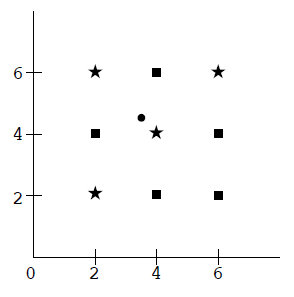
\includegraphics[height=5cm, keepaspectratio]{./dsc_255_hw1_5.png}
\end{center}

(a) \textit{How will the point be classified by 1-NN? The options are square, star, or ambiguous.}

(b) \textit{By 3-NN?}

(c) \textit{By 5-NN?}\\


\textbf{Solution (a)}

\noindent\rule{\textwidth}{0.4pt}\\

We know the point $p$ is located at $(3.5,4.5)$ and from the picture we are given the following:

$$\begin{bmatrix}\star_{(2,6)} & \blacksquare_{(4,6)} & \star_{(6,6)} \\ \blacksquare_{(2,4)} & \star_{(4,4)} & \blacksquare_{(6,4)} \\ \star_{(2,2)} & \blacksquare_{(4,2)} & \blacksquare_{(6,2)}\end{bmatrix}$$

The distance equation is given below:

$$\|x-y\| = \sqrt{\sum_{i=1}^{n} (x_i - y_i)^2}$$
\newpage
Now solve for the distance each element is away from point $p$


\begin{align*}
\|p - \star_{(2,6)}\| &= \sqrt{\left((3.5 - 2)^2 + (4.5 - 6)^2\right)} = \sqrt{\left((1.5)^2 + (-1.5)^2\right)} &\approx 2.12 \\
\|p - \blacksquare_{(4,6)}\| &= \sqrt{\left((3.5 - 4)^2 + (4.5 - 6)^2\right)} = \sqrt{\left((-0.5)^2 + (-1.5)^2\right)} &\approx 1.58 \\
\|p - \star_{(6,6)}\| &= \sqrt{\left((3.5 - 6)^2 + (4.5 - 6)^2\right)} = \sqrt{\left((-2.5)^2 + (-1.5)^2\right)} &\approx 2.92 \\
\|p - \blacksquare_{(2,4)}\| &= \sqrt{\left((3.5 - 2)^2 + (4.5 - 4)^2\right)} = \sqrt{\left((1.5)^2 + (0.5)^2\right)} &\approx 1.58 \\
\|p - \star_{(4,4)}\| &= \sqrt{\left((3.5 - 4)^2 + (4.5 - 4)^2\right)} = \sqrt{\left((-0.5)^2 + (0.5)^2\right)} &\approx 0.71 \\
\|p - \blacksquare_{(6,4)}\| &= \sqrt{\left((3.5 - 6)^2 + (4.5 - 4)^2\right)} = \sqrt{\left((2.5)^2 + (0.5)^2\right)} &\approx 2.55 \\
\|p - \star_{(2,2)}\| &= \sqrt{\left((3.5 - 2)^2 + (4.5 - 2)^2\right)} = \sqrt{\left((1.5)^2 + (2.5)^2\right)} &\approx 2.92 \\
\|p - \blacksquare_{(4,2)}\| &= \sqrt{\left((3.5 - 4)^2 + (4.5 - 2)^2\right)} = \sqrt{\left((-0.5)^2 + (2.5)^2\right)} &\approx 2.55 \\
\|p - \blacksquare_{(6,2)}\| &= \sqrt{\left((3.5 - 6)^2 + (4.5 - 2)^2\right)} = \sqrt{\left((2.5)^2 + (2.5)^2\right)} &\approx 3.54
\end{align*}

   
The distance results are below in \textit{Table 1}.
   
\begin{center}
\begin{tabular}{|c|c|c|}
\hline
Element & Distance to $p$ & Distance Rank \\
\hline
$\star_{(4,4)}$ & $0.71$ & $1^{st}$ \\
$\blacksquare_{(2,4)}$ & $1.58$ & $T2^{nd}$ \\
$\blacksquare_{(4,6)}$ & $1.58$ & $T2^{nd}$ \\
$\star_{(2,6)}$ & $2.12$ & $4^{th}$ \\
$\blacksquare_{(4,2)}$ & $2.55$ & $T5^{th}$ \\
$\blacksquare_{(6,4)}$ & $2.55$ & $T5^{th}$ \\
$\star_{(2,2)}$ & $2.92$ & $T7^{th}$ \\
$\star_{(6,6)}$ & $2.92$ & $T7^{th}$ \\
$\blacksquare_{(6,2)}$ & $3.54$ & $9^{th}$ \\
\hline
\end{tabular}
\end{center}

\textit{Table 1: ranking element distance to point p, closest to farthest}\\

From \textit{Table 1} $\star_{(4,4)}$ is closest to point $p$.

$\therefore$ the point $p$ will be classified as a star ($\star$) by 1-NN.

\noindent\rule{\textwidth}{0.4pt}\\  

\textbf{Solution (b)} 

\noindent\rule{\textwidth}{0.4pt}\\

\parbox{\textwidth}{From \textit{Table 1} in \textit{Solution (a)} the three elements closest to the point $p$ are:}\\ 

$$\star_{(4,4)} ,\blacksquare_{(2,4)} ,\blacksquare_{(4,6)}$$\\ 

\parbox{\textwidth}{The frequency counts are as follows: $\blacksquare : 2$ and $\star : 1$.}\\

$\therefore$ the point $p$ will be classified as a square ($\blacksquare$) by 3-NN.

\noindent\rule{\textwidth}{0.4pt}\\
\newpage
\textbf{Solution (c)} 

\noindent\rule{\textwidth}{0.4pt}\\

\parbox{\textwidth}{Again from \textit{Table 1} in \textit{Solution (a)} the five elements closest to the point $p$ are:}\\

$$\star_{(4,4)} ,\blacksquare_{(2,4)} ,\blacksquare_{(4,6)} ,\star_{(2,6)} ,\blacksquare_{(4,2)} | \blacksquare_{(6,4)}$$ \\

\parbox{\textwidth}{The frequency counts are as follows: $\blacksquare : 3$ and $\star : 2$.}\\

$\therefore$ the point $p$ will be classified as a square ($\blacksquare$) by 5-NN.

\noindent\rule{\textwidth}{0.4pt}

\noindent\rule{\textwidth}{0.4pt}

\subsection*{Question 6}
\textit{We decide to use 4-fold cross-validation to figure out the right value of $k$ to choose when running $k$-nearest neighbor on a data set of size 10,000. When checking a particular value of $k$, we look at four different training sets. What is the size of each of these training sets?}\\

\textbf{Solution} 

\noindent\rule{\textwidth}{0.4pt}\\

Let, $k=4$ and $n=10000$

Calculate the size of each fold ($f_s$).

$f_s = \frac{n}{k} = \frac{10000}{4} = 2500$

Hence, the size of each fold is $2500$

Now, we will solve for the size of each training set ($t_s$) using the equation below:

$$t_s = (k-1)\times f_s$$

Calculate the size of each training set such that $f_s=2500$ and $k=4$.

$t_s = (k-1)\times f_s = (4-1) \times 2500 = 7500$\\

$\therefore$ the size of each training set is $7500$

\noindent\rule{\textwidth}{0.4pt}

\noindent\rule{\textwidth}{0.4pt}

\subsection*{Question 7}

\textit{An extremal type of cross-validation is $n$-fold cross-validation on a training set of size $n$. If we want to estimate the error of $k$-NN, this amounts to classifying each training point by running $k$-NN on the remaining $n-1$ points, and then looking at the fraction of mistakes made. It is commonly called leave-one-out cross-validation (LOOCV).}

\textit{Consider the following simple data set of just four points:}

\begin{center}
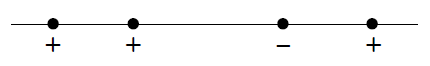
\includegraphics[width=0.7\textwidth]{dsc_255_hw1_7.png}
\end{center}

\textit{What is the LOOCV error for:}
\begin{itemize}
    \item 1-NN
    \item 3-NN
\end{itemize}

\textbf{Solution}

\noindent\rule{\textwidth}{0.4pt}\\

Let the points seen above be defined as the following:

$$p_1 = +$$
$$p_2 = +$$
$$p_3 = -$$
$$p_4 = +$$

\begin{itemize}
    \item LOOCV error for 1-NN
\end{itemize}


Each $p_i$ for 1-NN would be classified as follows

\begin{center}
\begin{tabular}{|c|c|c|c|}
\hline
Point & Nearest Neighbor & Classification & Prediction \\
\hline
$p_1(+)$ & $p_2(+)$ & $+$ & $True$ \\
$p_2(+)$ & $p_1(+)$ & $+$ & $True$ \\
$p_3(-)$ & $p_4(+)$ & $+$ & $False$ \\
$p_4(+)$ & $p_3(-)$ & $-$ & $False$ \\
\hline
\end{tabular}
\end{center}

From the table above we have two correct predictions for the four points or an accuracy of $50\%$.

Now , calculate LOOCV error ($LOOCV_{error}$)

$LOOCV_{error} = 1 - accuracy = 1 - 0.50 = 0.50$\\

$\therefore$ LOOCV error for 1-NN is $50\%$.

\noindent\rule{\textwidth}{0.4pt}

\begin{itemize}
    \item LOOCV error for 3-NN
\end{itemize}

Each $p_i$ for 3-NN would be classified as follows

\begin{center}
\begin{tabular}{|c|c|c|c|c|}
\hline
Point & Nearest Neighbors & Majority & Classification & Prediction \\ 
\hline
$p_1(+)$ & $p_2(+)$ , $p_3(-)$ , $p_4(+)$ & $+$ & $+$ & $True$ \\
$p_2(+)$ & $p_1(+)$ , $p_3(-)$ , $p_4(+)$ & $+$ & $+$ & $True$ \\
$p_3(-)$ & $p_1(+)$ , $p_2(+)$ , $p_4(+)$ & $+$ & $+$ & $False$ \\
$p_4(+)$ & $p_1(+)$ , $p_2(+)$ , $p_3(-)$ & $+$ & $+$ & $True$ \\
\hline
\end{tabular}
\end{center}

From the table above we have three correct predictions for the four points

Now , calculate LOOCV error ($LOOCV_{error}$)

$LOOCV_{error} = 1 - accuracy = 1 - 0.75 = 0.25$

$\therefore$ LOOCV error for 3-NN is $25\%$.

\noindent\rule{\textwidth}{0.4pt}
\noindent\rule{\textwidth}{0.4pt}

\subsection*{Programming Exercises}

\textit{Before attempting this problem, make sure that Python 3 and Jupyter are installed on your computer.}
\subsection*{Question 8}

\textit{\textbf{Nearest neighbor on MNIST.} For this problem, download the archive \texttt{hw1.zip}, available from the course website, and open it. The Jupyter notebook \texttt{nn-mnist.ipynb} implements a basic 1-NN classifier for a subset of the MNIST data set. It uses a separate training and test set. Begin by going through this notebook, running each segment and taking care to understand exactly what each line is doing.}

\begin{enumerate}[label=(a)]
  \item \textit{For test point 100, print its image as well as the image of its nearest neighbor in the training set. Put these images in your writeup. Is this test point classified correctly?}
\end{enumerate}
\begin{enumerate}[label=(b)]
  \item \textit{The confusion matrix for the classifier is a $10 \times 10$ matrix $N_{ij}$ with $0 \leq i, j \leq 9$, where $N_{ij}$ is the number of test points whose true label is $i$ but which are classified as $j$. Thus, if all test points are correctly classified, the off-diagonal entries of the matrix will be zero.}
  \begin{itemize}
      \item \textit{Compute the matrix $N$ for the 1-NN classifier and print it out.}
      \item \textit{Which digit is misclassified most often? Least often?}
  \end{itemize}
\end{enumerate}
\begin{enumerate}[label=(c)]
  \item \textit{For each digit $0 \leq i \leq 9$,: look at all training instances of image i, and compute their mean. This average is a 784-dimensional vector. Use the show digit routine to print out these 10 average-digits.}\\
\end{enumerate}

\textbf{Solution (a)}

\noindent\rule{\textwidth}{0.4pt}\\

\parbox{\textwidth}{In order to print the $100^{th}$ test point image, its nearest neighbor in the training set, and classification from the Jupyter notebook \texttt{nn-mnist.ipynb} we must use the following function:}\\

Functions for printing the test point and training image:\\
\begin{center}

\begin{lstlisting}
## Define a function that displays a digit given its vector representation
def show_digit(x):
    plt.axis('off')
    plt.imshow(x.reshape((28,28)), cmap=plt.cm.gray)
    plt.show()
    return

## Define a function that takes an index into a particular data set ("train" or "test") and displays that image.
def vis_image(index, dataset="train"):
    if(dataset=="train"): 
        show_digit(train_data[index,])
        label = train_labels[index]
    else:
        show_digit(test_data[index,])
        label = test_labels[index]
    print("Label " + str(label))
    return

## Takes a vector x and returns the index of its nearest neighbor in train_data
def find_NN(x):
    # Compute distances from x to every row in train_data
    distances = [squared_dist(x,train_data[i,]) for i in range(len(train_labels))]
    # Get the index of the smallest distance
    return np.argmin(distances)

## Takes a vector x and returns the class of its nearest neighbor in train_data
def NN_classifier(x):
    # Get the index of the the nearest neighbor
    index = find_NN(x)
    # Return its class
    return train_labels[index]

\end{lstlisting}
    
\end{center}
\newpage
\parbox{\textwidth}{Print the $100^{th}$ test point image, print the $100^{th}$ test point's NN in the training set, and determine if the classification is correct:}\\
\begin{center}

\begin{lstlisting}
## View the 100th data point in the test set
vis_image(99, "test")

## Find index of NN for the 100th data point in the test set
index_NN = find_NN(test_data[99,])
print("Nearest neighbor index: ", index_NN)

## View the nearest neighbor for the 100th data point in the training set
vis_image(index_NN, "train")

## Classify the 100th data point in the test set
print("Predicted label: ", NN_classifier(test_data[99,]))

## Check the true label of the 100th data point in the test set
print("True label: ", test_labels[99])

\end{lstlisting}

\begin{figure}[htbp]
\centering
\begin{tabular}{>{\centering\arraybackslash}p{0.4\textwidth} >{\centering\arraybackslash}p{0.4\textwidth}}
$100^{th}$ test point image & NN \\
\includegraphics[width=0.4\textwidth]{dsc_255_hw1_8_test_100.png} & \includegraphics[width=0.4\textwidth]{dsc_255_hw1_8_test_100_nn.png} \\
\end{tabular}
\caption{Comparison of 100th test point and its nearest neighbor.}
\label{fig:image_comparison}
\end{figure}
    
\end{center}

\parbox{\textwidth}{The predicted and true label was 8.}\\

\parbox{\textwidth}{$\therefore$ the $100^{th}$ test point was classified correctly.}\\

\noindent\rule{\textwidth}{0.4pt}\\
\newpage
\textbf{Solution (b)}

\noindent\rule{\textwidth}{0.4pt}

\begin{itemize}
    \item \textit{Compute the matrix $N$ for the 1-NN classifier and print it out.}
\end{itemize}

\parbox{\textwidth}{Python code used to compute the matrix $N$ for the 1-NN classifier (\textit{confusion matrix}), print the confusion matrix and visualize the confusion matrix.}\\
\begin{center}

\begin{lstlisting}
## Import libraries for hw1_q8_b
from sklearn.metrics import confusion_matrix
import seaborn as sns
import numpy as np
import matplotlib.pyplot as plt

## Define test predictions and test labels
test_predictions = [NN_classifier(test_data[i,]) for i in range(len(test_labels))]
test_labels = np.load('MNIST/test_labels.npy')

## Use sklearn to compute the confusion matrix
N_train = confusion_matrix(test_predictions, test_labels)

## Print the confusion matrix
print("Confusion Matrix for 1-NN classifier on test set:")
print(N_train)

## Visualize the confusion matrix using a heatmap
plt.figure(figsize=(10, 8))
sns.heatmap(N_train, annot=True, fmt='d', cmap=sns.color_palette("rocket", as_cmap=True))
plt.xlabel('Predicted Label')
plt.ylabel('True Label')
plt.title('Confusion Matrix for 1-NN Classifier on MNIST Training Set')
plt.show()
\end{lstlisting}

\end{center}

\begin{figure}[htbp]
\centering
\begin{minipage}{0.48\textwidth} % Adjust width as needed
  \centering
  Printed Confusion Matrix \\
  \includegraphics[width=\textwidth]{dsc_255_hw1_8_cm_print.png}
  \caption{Printed confusion matrix $N$ via Python.}
  \label{fig:image_comparison_1}
\end{minipage}\hfill % Add horizontal space
\begin{minipage}{0.48\textwidth} % Adjust width as needed
  \centering
  Visualization \\
  \includegraphics[width=\textwidth]{dsc_255_hw1_8_cm.png}
  \caption{Visualization of confusion matrix $N$.}
  \label{fig:image_comparison_2}
\end{minipage}
\end{figure}

\begin{itemize}
    \item \textit{Which digit is misclassified most often? Least often?}
\end{itemize}

\parbox{\textwidth}{From \textit{Figure 3}, we want to find the minimum and maximum values along the diagonal. The minimum value along the diagonal represents the digit that is misclassified most often. Conversely, the maximum value along the diagonal represents the digit that is misclassified least often. Please note this max/min rule of thumb is only true when we have equal frequencies of each label.}\\

$\therefore$ the digit \textit{9} is misclassified most often and the digit \textit{1} is misclassified least often.\\
\noindent\rule{\textwidth}{0.4pt}\\
\newpage

\textbf{Solution (c)}

\noindent\rule{\textwidth}{0.4pt}\\

\parbox{\textwidth}{Python code used to compute average digit images and display them using the \textbf{show\_digit} function in the Jupyter notebook \texttt{nn-mnist.ipynb} }

\begin{center}

\begin{lstlisting}
## Get unique digits in the training set
unique_digits = np.unique(train_labels, return_counts=False)

## Initialize a dictionary to hold the digit image arrays
unique_digit_image_arrays = {i:[] for i in unique_digits}

## Initialize a dictionary to hold the average digit images
average_digits = {i:'' for i in unique_digits}

## Append each digit image to the corresponding list in the dictionary
for label_index in range(train_labels.shape[0]):
    unique_digit_image_arrays[train_labels[label_index]].append(train_data[label_index])

## Compute the average digit images and display them using show_digit
for label in average_digits:
    combined = np.stack(tuple(unique_digit_image_arrays[label]))
    average_digits[label] = np.mean(combined, axis=0)
    show_digit(average_digits[label])

\end{lstlisting}
\end{center}

\begin{figure}[htbp]
\centering
\begin{tabular}{>{\centering\arraybackslash}p{0.4\textwidth} >{\centering\arraybackslash}p{0.4\textwidth}}
$0$ Label & $1$ Label \\
\includegraphics[width=0.4\textwidth]{dsc_255_hw1_8_0_avg.png} & \includegraphics[width=0.4\textwidth]{dsc_255_hw1_8_1_avg.png} \\
\end{tabular}
\caption{Average image for the zero and one label.}
\label{fig:image_comparison}
\end{figure}

\begin{figure}[htbp]
\centering
\begin{tabular}{>{\centering\arraybackslash}p{0.4\textwidth} >{\centering\arraybackslash}p{0.4\textwidth}}
$2$ Label & $3$ Label \\
\includegraphics[width=0.4\textwidth]{dsc_255_hw1_8_2_avg.png} & \includegraphics[width=0.4\textwidth]{dsc_255_hw1_8_3_avg.png} \\
\end{tabular}
\caption{Average image for the two and three label.}
\label{fig:image_comparison}
\end{figure}

\begin{figure}[htbp]
\centering
\begin{tabular}{>{\centering\arraybackslash}p{0.4\textwidth} >{\centering\arraybackslash}p{0.4\textwidth}}
$4$ Label & $5$ Label \\
\includegraphics[width=0.4\textwidth]{dsc_255_hw1_8_4_avg.png} & \includegraphics[width=0.4\textwidth]{dsc_255_hw1_8_5_avg.png} \\
\end{tabular}
\caption{Average image for the four and five label.}
\label{fig:image_comparison}
\end{figure}

\begin{figure}[htbp]
\centering
\begin{tabular}{>{\centering\arraybackslash}p{0.4\textwidth} >{\centering\arraybackslash}p{0.4\textwidth}}
$6$ Label & $7$ Label \\
\includegraphics[width=0.4\textwidth]{dsc_255_hw1_8_6_avg.png} & \includegraphics[width=0.4\textwidth]{dsc_255_hw1_8_7_avg.png} \\
\end{tabular}
\caption{Average image for the six and seven label.}
\label{fig:image_comparison}
\end{figure}

\begin{figure}[htbp]
\centering
\begin{tabular}{>{\centering\arraybackslash}p{0.4\textwidth} >{\centering\arraybackslash}p{0.4\textwidth}}
$8$ Label & $9$ Label \\
\includegraphics[width=0.4\textwidth]{dsc_255_hw1_8_8_avg.png} & \includegraphics[width=0.4\textwidth]{dsc_255_hw1_8_9_avg.png} \\
\end{tabular}
\caption{Average image for the eight and nine label.}
\label{fig:image_comparison}
\end{figure}

\end{document}

